\textit{This chapter describes work that is still in progress, and that was done during an academic visit with Pr Edoardo Ponti at the University of Edinburgh.}

\vspace{1em}

\Cref{chap:anisotropy} shows that studying the representation degeneration phenomenon at self-attention level sheds light on the sparse nature of most attention maps. It depicts a connection between anisotropy and sparsity in the attention maps of language models, as the identified common drift direction is used to encode the selective process of a specific head.

This observation raises questions about the efficiency of the attention operation, as most of the attention values are actually not relevant in the production of the output of the self-attention layer. It also questions the effect of such sparsity requirements on the upstream latent spaces of these language models, and on the possible harmfulness of the distortions that affect them.

\begin{figure}[!b]
    \centering
    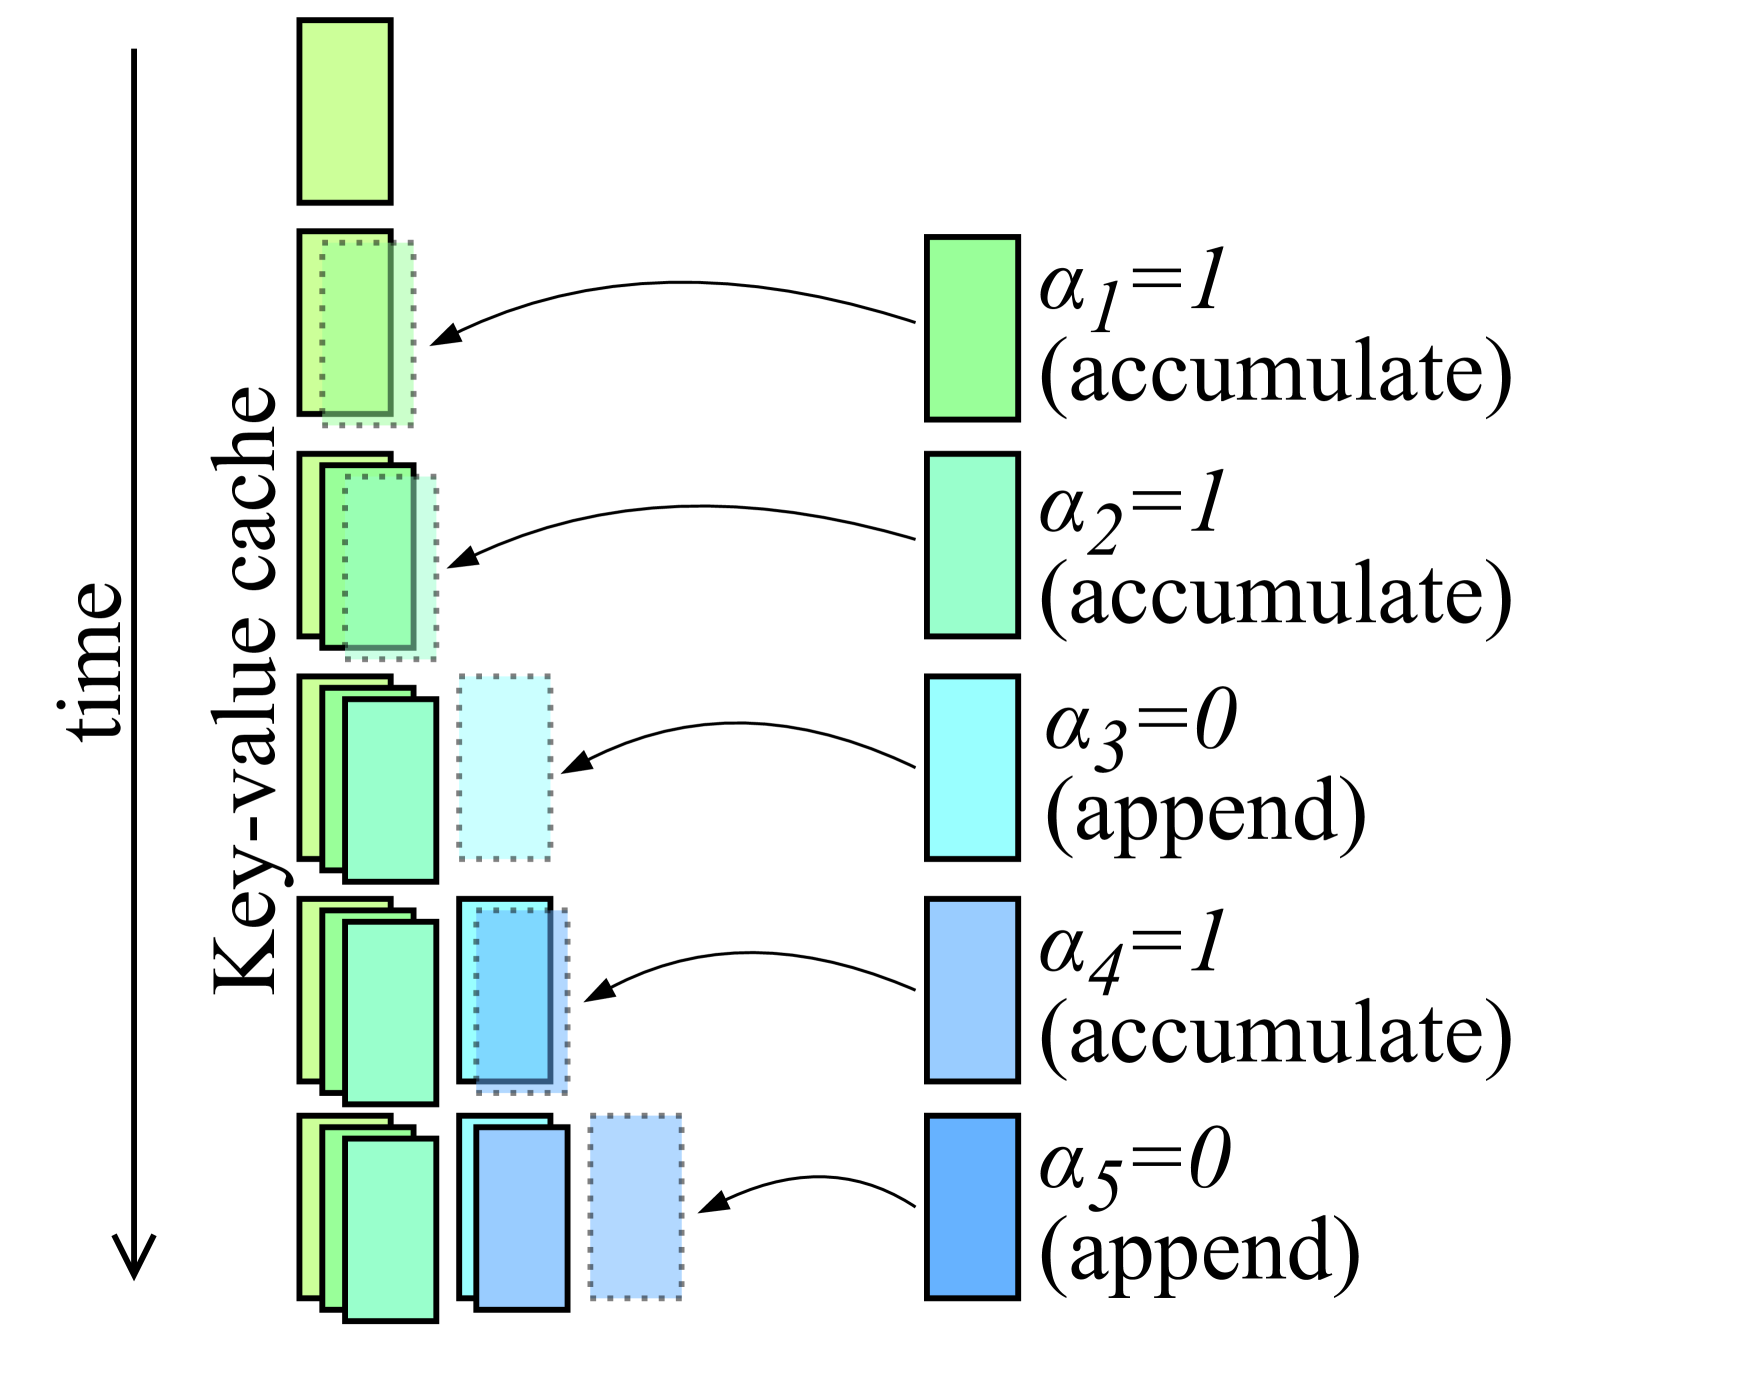
\includegraphics[width=0.6\linewidth]{sources/part_2/kv_cache/imgs/dmc_schema.png}
    \caption{Schema of the Dynamic Memory Compression technique from \citep{nawrot2024dynamic}. A merge decision is made at every step, which either extends the KV cache with a new slot or adds the current KV representations into the current slot. During training, the Gumbel reparameterization trick allows to mimic sampling the merge decision in a differentiable manner.}
    \label{fig:dmc_schema}
\end{figure}

As mentioned in \Cref{ssec:efficient_attn}, several works have explored ways to reduce the sparsity of self-attention maps, by filtering the $(i, j)$ index pairs where attention should be computed during training and inference, in order to reduce the time and memory complexity of self-attention. Another line-of-work proposes solutions that focus on post-training efficiency improvement and build heuristics that minimize the impact of removing $K^h$ and $V^h$ representations on performance, earning these methods the name of Key-Value (KV) cache compression. 

Limitations of most KV cache compression schemes include that the heuristics are hand-crafted and may thus be suboptimal, but also that these methods are non-differentiable and cannot be used as efficient attention methods to train models from scratch.

\citet{nawrot2024dynamic} overcome this differentiability limitation by using a Gumbel-sigmoid activation on top of the first coefficients of $Q^h$ and $K^h$ to predict a decision to merge into the current cache slot or to create a new cache slot. Thanks to this technique, the authors are able to continue the training of language models with an auxiliary objective that measures the compression ratio and optimize the KV cache size while retaining the language modeling performance.

The Gumbel reparameterization trick \citep{jang2017categorical} allows to mimic multinomial sampling in a differentiable manner, which is useful in models that require to emulate such sampling during training. Nevertheless, these methods add stochastic noise to their input, which may alter the expressiveness of gradients. Moreover, \citet{nawrot2024dynamic} only consider contiguous compression, where only representations corresponding to contiguous positions can be merged, which restricts the expressiveness of the compression scheme.

In this chapter, we provide ideas and experiments towards extending the dynamic KV cache compression method of \citet{nawrot2024dynamic}. Notably, we provide a mathematical framework for neural compressive methods in the causal setting without sampling via methods based on the Gumbel reparameterization trick. We test our framework by training causal models with compressive attention from scratch, and by continue-training models for KV cache compression.


\section{Mathematical framework}

We propose to lay the foundations for an efficient causal compressive attention module, based on basic matrix operations. For the sake of simplicity, we consider a basic single-head attention setup with input representations $Q, K, V \in \mathbb{R}^{L \times d_m}$, and without output projection $W_O$.

We recall from \Cref{ssec:transformers} the expression of the attention map $A$ and of the attention output $v$:
\begin{equation}
\begin{cases}
A = \sigma \left(\frac{Q K^T}{\sqrt{d_h}} + \mathcal{M} \right) \\
v = AV
\end{cases}
\label{eq:attn_sing_head}
\end{equation}
where $\sigma$ is the softmax function applied to the last dimension, $\mathcal{M}$ is the causal mask and $d_h=d_m$ as there is only one head.

We view compression as a matrix multiplication based on a \textit{compression mapping} $M \in \mathbb{R}^{L_C \times L}$, with $L_C \leq L$. Ideally, we want to build compressed views of $K$ and $V$ in $\mathbb{R}^{L_C \times d_m}$ by computing:
\begin{equation*}
\begin{cases}
K_C = M K \\
V_C = M V
\end{cases}
\end{equation*}
and using $K_C$ and $V_C$ instead of $K$ and $V$ in the self-attention operations described in \Cref{eq:attn_sing_head}.

This approach leads to an immediate complication with respect to causality, as the product $QK_C^T$ allows for non-causal interactions, i.e. operations between features from $Q_i$ and $K_j$ where $i > j$. A similar problem occurs in the $AV_C$ product. We propose to overcome this issue by first remarking that 
$$QK_C^T = Q(MK)^T = (QK^T)M^T$$
and
$$AV_C = (AM)V$$

Hence, it is possible to cancel the influence of non-causal interactions before compression by nulling out the corresponding coordinates using a binary causal mask $$\mathcal{M}_1 = \exp \mathcal{M}$$which is basically a lower triangular matrix filled with $1$. For instance, the query-key product can be rewritten as $(QK^T \odot \mathcal{M}_1) M^T$ where $\odot$ is the element-wise product.

Although this trick solves causality issues, it also makes the causal mask $\mathcal{M}$ inaccurate with respect to the softmax function $\sigma$. Indeed, in \Cref{eq:attn_sing_head}, $\mathcal{M}$ removes attention map indices that do not respect causality from the computation of the softmax. In the compressed sequence scenario, and especially when $M$ is sparse, these indices can be found in positions $(i,j)$ where the compression mapping only pools from positions after $i$ into position $j$, i.e. where $\left(\mathcal{M}_1 M^T\right)_{ij} = 0$.

We can thus design a causal mask for softmax $\mathcal{M_C}$ that takes compression into account:
$$
\mathcal{M}_C = \log \mathbf{1}_{\mathcal{M}_1 M^T > 0}
$$

We can now formulate a compressed version of causal self-attention:

\begin{equation}
\begin{cases}
A = \sigma \left(\left(\frac{Q K^T}{\sqrt{d_h}} \odot \mathcal{M}_1\right) M^T + \mathcal{M}_C \right) \\
v = \left(AM \odot \mathcal{M}_1\right)V
\end{cases}
\label{eq:comp_attn_sing_head}
\end{equation}

\begin{figure}[!ht]
    \centering
    \begin{subfigure}[b]{0.48\columnwidth}
         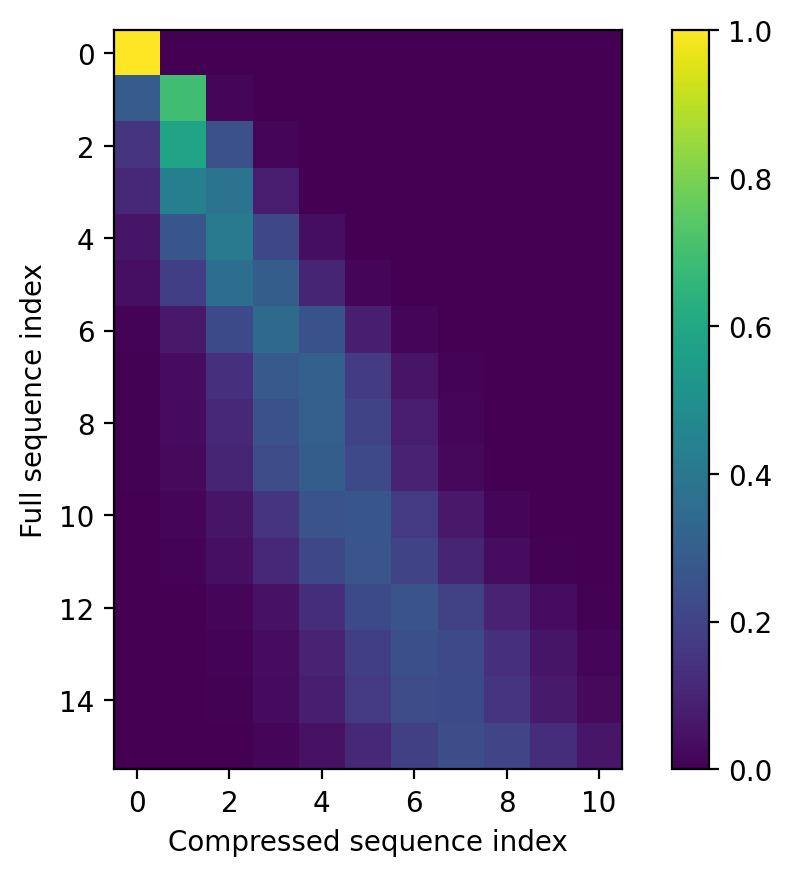
\includegraphics[width=\linewidth]{sources/part_2/kv_cache/imgs/compression_map_ex.png}
         \caption{Compression mapping $M$}
    \end{subfigure}
    \begin{subfigure}[b]{0.39\columnwidth}
         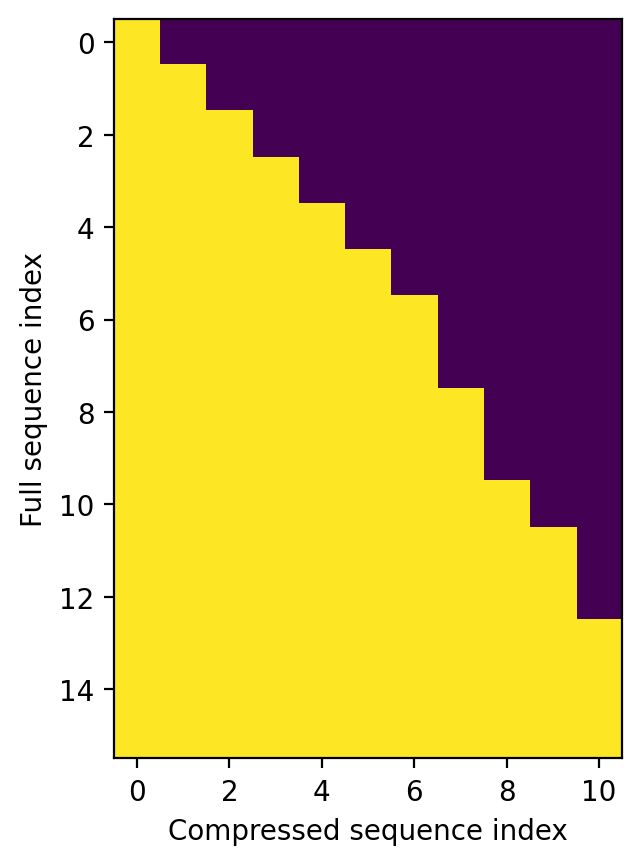
\includegraphics[width=\linewidth]{sources/part_2/kv_cache/imgs/compressed_M_C_ex.png}
         \caption{Softmax mask $\mathcal{M}_C$}
    \end{subfigure}
    \begin{subfigure}[b]{0.48\columnwidth}
         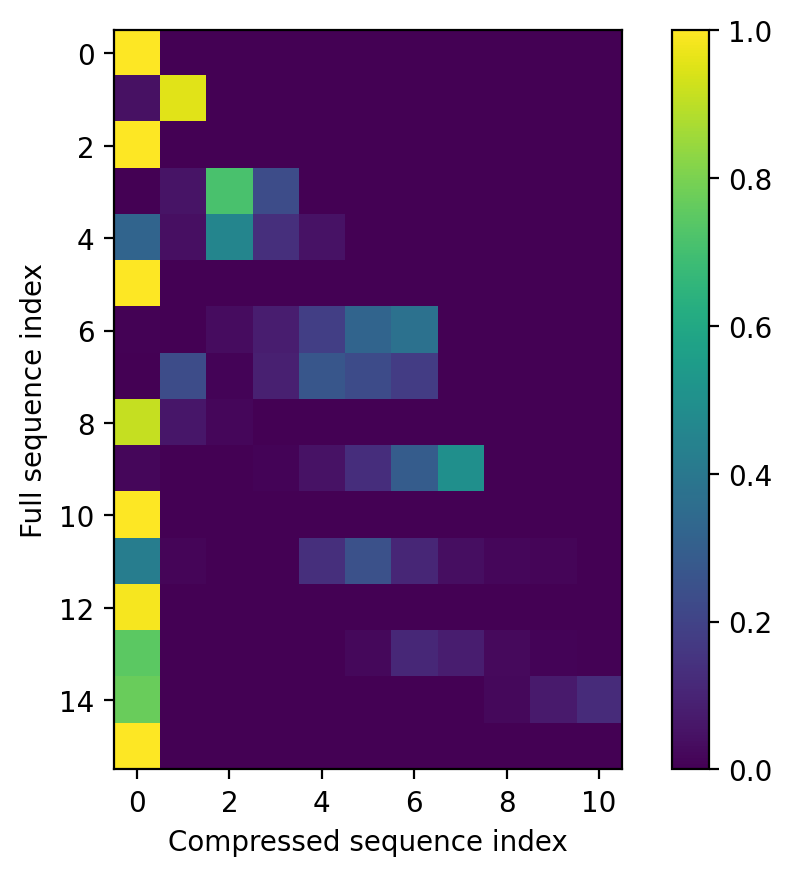
\includegraphics[width=\linewidth]{sources/part_2/kv_cache/imgs/compressed_attn_map_ex.png}
         \caption{Attention map $A$}
    \end{subfigure}
    
    \caption{An example of compressed attention with random input representations and using the MANTa mapping to build $M$.}
    \label{fig:formula_viz_dmc}
\end{figure}

To extend this framework to multi-head attention, the operation described in \Cref{eq:comp_attn_sing_head} can be computed for all heads, each head potentially applying a different compression mapping.

\section{Predicting compression mappings}
The interest of \Cref{eq:comp_attn_sing_head} lies in the fact that \textit{any} compression mapping $M \in \mathbb{R}^{L_C \times L}$ can be used. This includes static compression mappings, parameterized matrices, or even the results of parameterized operations on $Q$, $K$, and/or $V$ representations.

In this chapter, we particularly focus on compression maps that are well-suited for KV cache compression, which restrains design choices to compression maps that are built in a causal way themselves, as the cached $K_C$ and $V_C$ representations can only be updated using the currently available representations at generation step $t$, which includes $K_t$, $V_t$ and $K_C$ and $V_C$ themselves.

Consequently, a natural choice is to adapt our work on the MANTa module in \Cref{chap:manta} to this framework. We call $\Psi$ the function that maps frontier decisions $p_{F_t}$ to the Gaussian kernel used to approximate the Poisson-binomial distribution in \Cref{ssec:manta_maths}. As the intermediate representations of Transformer-based models are already contextualized and contain positional information, except for the first layer, we do not need a contextualizing module to obtain $p_{F_t}$, or a convolution to encode position when pooling representations. 

Following \citet{nawrot2024dynamic}, we also implement a weighting mechanism that allows to discard representations altogether, and to weight contributions in the pooled representations. 

Formally, in the single head scenario, we introduce two linear layers of weights $W_F$ and $W_\omega$ in $\mathbb{R}^{3d_m \times 1}$ that are applied to $\{QKV\} \in \mathbb{R}^{L \times 3d_m}$, the concatenation of $Q$, $K$ and $V$ in the feature dimension. The compression mapping is then computed as:
\begin{equation}
    \begin{cases}
        p_F = \varsigma \left(\{QKV\} W_F + C_F\right) \\
        \Omega = \varsigma \left(\{QKV\} W_\omega + C_\omega\right) \\
        M = \Psi(p_F) \odot \Omega
    \end{cases}
\end{equation}
where $\varsigma$ is the sigmoid function, and $C_F$ and $C_\omega$ are constants that help initialize the model in a non-compressive way, i.e. where $p_F \approx\mathbf{1}$ and $\Omega \approx\mathbf{1}$ so that $M \approx I_L$.

As $\{QKV\}$ is computed in a causal fashion, $p_{F_t}$ and $\Omega_t$ are not affected by future positions of the sequence, and will not change when generating further in the sequence. Hence, the first $t$ columns of $M$ are not affected by $\{QKV\}_i$ when $i > t$. Moreover, $\Psi$ can easily be computed in a memory-efficient way at inference, by storing the running average and variance for block position as $t$ increases. This implies that the parallel computation of compressed self-attention in Transformer blocks can easily be adapted to an efficient KV caching system during inference.

Similarly to \citet{nawrot2024dynamic}, we train language models with an auxiliary loss that measures the average compression rate:
$$
\mathcal{L}_C = \frac{1}{L} \sum_{t=1}^L p_{F_t}
$$

The global loss of the model is then defined as:
$$
\mathcal{L} = \mathcal{L}_{ce} + \lambda_{C} \mathcal{L}_C
$$


\section{Preliminary experiments}

In this section, we provide some of the first results we obtained with the method described in previous sections. This work still being in progress, we warn the reader that these results constitute proofs-of-concept rather than strong results that would allow conclusive statements about the method.

\subsection{Pretraining}

We train 70 million parameter models using the same architecture as its Pythia counterpart \citep{pythia} on the CCNews \citep{Hamborg2017} dataset. We use small batch sizes of 32 sequences of length 128 to accelerate training. We perform 100,000 steps, which represents 409M tokens. The weights are optimized using AdamW with no weight decay and a learning rate of $10^{-3}$ for all parameters except $W_F$ and $W_\omega$ for which a learning rate of $10^{-4}$ is used, accordingly with \Cref{chap:manta}. We also use a cosine scheduling with a 2000-step warm up phase. We set $C_F = C_\omega = 5$ to make sure the model starts with a compression ratio close to $1$. We observe that training throughput is not significantly affected by the compression operation, when using a pure PyTorch implementation of self-attention.

We explore values of $\lambda_C$ in $\{1 \cdot 10^{-2}, 2 \cdot 10^{-2}, 3 \cdot 10^{-2}\}$ leading to different final compression ratios, as pictured in \Cref{fig:train_dmc_cr}.

\begin{figure}[!ht]
    \centering
    \begin{subfigure}[b]{0.6\columnwidth}
         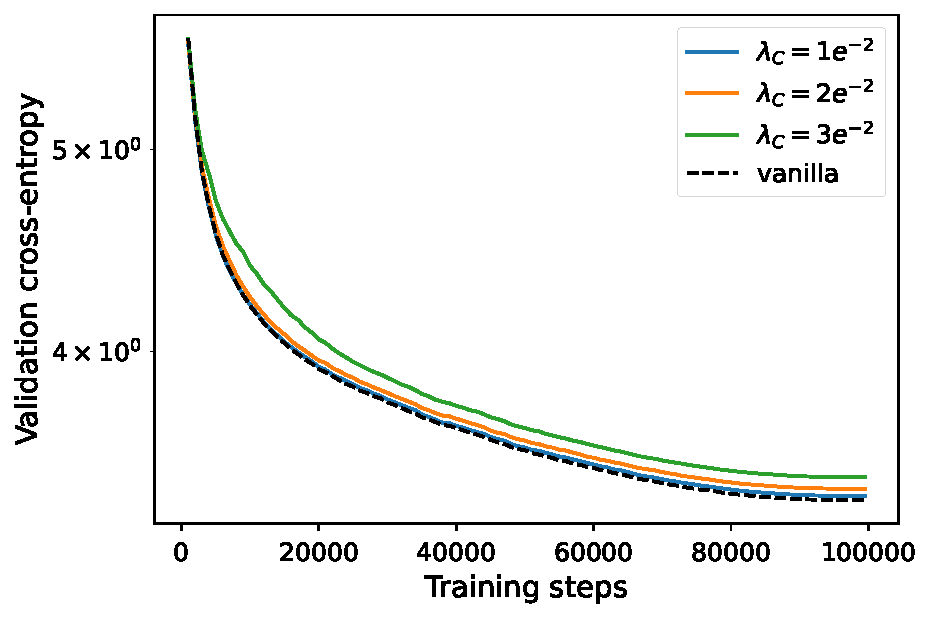
\includegraphics[width=\linewidth]{sources/part_2/kv_cache/imgs/ce_val.pdf}
         \caption{Validation LM loss}
    \end{subfigure}
    \begin{subfigure}[b]{0.6\columnwidth}
         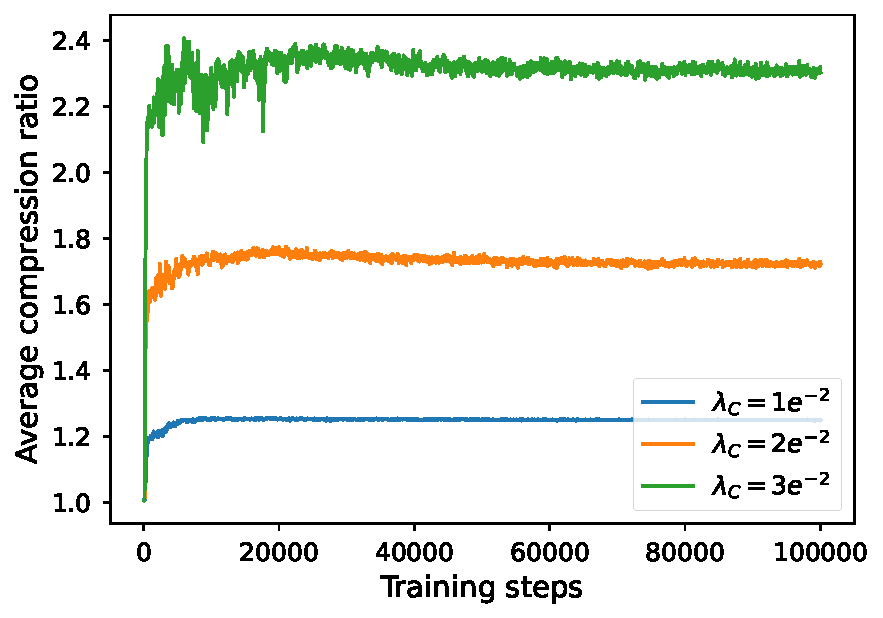
\includegraphics[width=\linewidth]{sources/part_2/kv_cache/imgs/comp_ratio.pdf}
         \caption{Compression ratio}
         \label{fig:train_dmc_cr}
    \end{subfigure}
    
    \caption{Training dynamics of our language models trained with compressed attention.}
    \label{fig:train_dmc}
\end{figure}

In \Cref{fig:comp_maps}, we show examples of learned compression maps for the model trained with $\lambda_C = 2 \cdot 10^{-2}$.

\begin{figure}[!ht]
    \centering
    \begin{subfigure}[b]{0.6\columnwidth}
         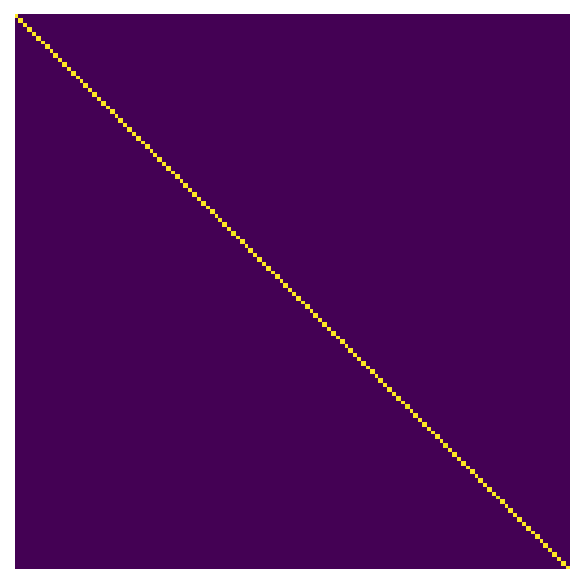
\includegraphics[width=\linewidth]{sources/part_2/kv_cache/imgs/layer1_head2.pdf}
         \caption{Layer 2, head 3}
    \end{subfigure}
    \begin{subfigure}[b]{0.6\columnwidth}
         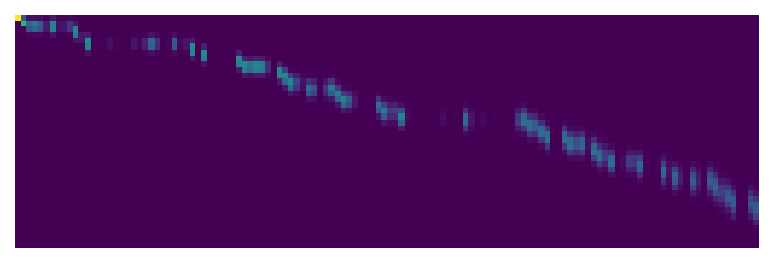
\includegraphics[width=\linewidth]{sources/part_2/kv_cache/imgs/layer3_head4.pdf}
         \caption{Layer 4, head 5}
    \end{subfigure}
    \begin{subfigure}[b]{0.6\columnwidth}
         
\includegraphics[width=\linewidth]{sources/part_2/kv_cache/imgs/layer5_head4.pdf}
         \caption{Layer 6, head 5}
    \end{subfigure}
    
    \caption{Compression maps $M$ for the final checkpoint of the model trained with $\lambda_C = 2 \cdot 10^{-2}$ (in transposed view)}
    \label{fig:comp_maps}
\end{figure}
% \FloatBarrier

\Cref{fig:comp_maps} depicts different compression schemes, with compression rates that increase as we move towards deeper layers. Overall, these experiments tend to demonstrate the potential of this approach, as it allows us to train models from scratch with compressed KV cache. 

We leave our initial hypothesis on the impact of denser attention maps on the anisotropy of intermediate layers for future work, as proving it would require using larger models trained in regular hyperparameter setups, these small models being extremely anisotropic regardless of the compression behavior.

\subsection{Application to KV cache compression}

We also apply our method to KV cache compression. To do so, we initialize our compressed attention architecture with the weights of a pretrained model of 160 million parameters from the Pythia suite, and choose sufficiently high values for $C_F$ and $C_\omega$ so that compression is minimal and the performance is retained. We perform an extensive hyperparameter search for this procedure, and report the results of this search in \Cref{fig:hp_search_kvc}.

\begin{figure}[!ht]
    \centering
     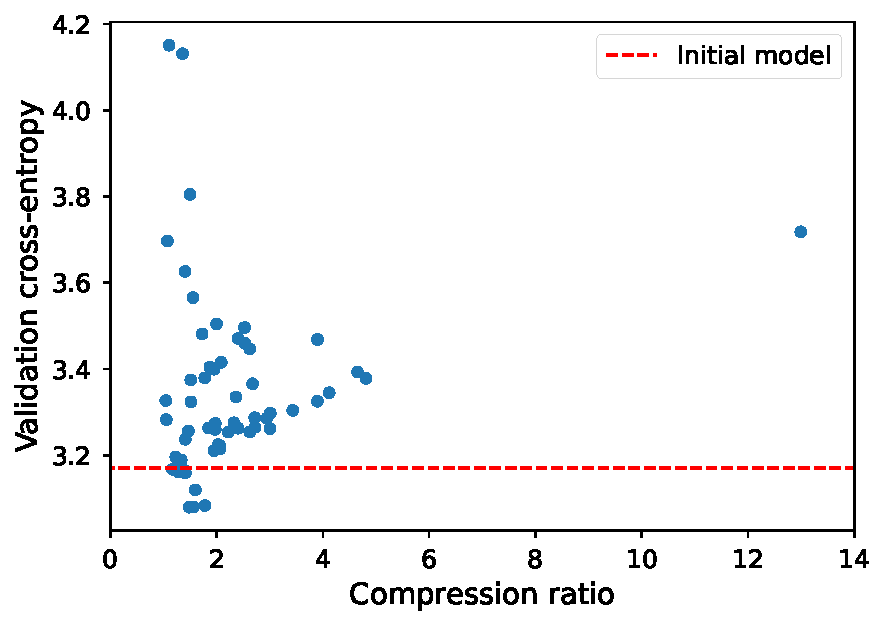
\includegraphics[width=0.6\linewidth]{sources/part_2/kv_cache/imgs/hp_search_kvc_160m.pdf}
    \caption{Results of our hyperparameter search on KV cache compression setups for a Pythia-160M. Each point represents a choice of hyperparameters.}
    \label{fig:hp_search_kvc}
\end{figure}

\Cref{fig:hp_search_kvc} illustrates the high sensitivity of this method to hyperparameter choices when applied to KV cache compression. Interestingly, we are able to reach a $13 \times$ compression ratio while retaining reasonable language modeling capabilities, and we also observe cases where the continued training of the model on the CCNews data led to improved performance while still achieving non-negligible compression levels.

This exploration incentivizes future research on improving the stability of continued training when using MANTa-based compression mappings.

\section*{Conclusion}

In this chapter, we introduce a mathematical framework for fully differentiable compression of keys and values in the self-attention operation, which implicitly densifies the attention maps used by the models, and allows more memory-efficient modeling. We notably design a way to solve the causality issue that emerges when conceiving such models by using several masks that filter out the non-causal interactions between sequential features.

We proceed to explore a specific family of compression mappings based on the MANTa module presented in \Cref{chap:manta}. We apply our method to causal language model pretraining and demonstrate the potential of our method by achieving $2 \times$ compression while retaining similar performance levels. We also present initial results on the KV cache compression setup, opening up challenging questions for future work.

This preliminary study could also lead to other types of compression mappings, which could include mappings based on a basis of cosine-based vectors to model long-range non-contiguous pooling, negative weight contributions to the compressed sequence to mimic a discarding operation at a later generation step, or fixed-length compression with unconstrained weights.

\vspace{2em}

This chapter paves the way for automatically learned dense attention maps through a novel mechanism for self-attention that allows to include a sequence-wise compression operation. Taking advantage of the sparsity of attention is a promising way towards more efficient language models.

As we discussed in \Cref{chap:anisotropy}, the sparsity of self-attention can also induce distortions in the latent space of queries and keys. We hypothesize that a sufficiently expressive compression mapping function could mitigate such phenomenon and allows for easier selective interactions while minimizing the resulting distortions. We leave the exploration of this hypothesis to future work.

